%%%%%%%%%%%%%%%%%%%%%%%%%%%%%%%%%%%%%%%%%
% Beamer Presentation
% LaTeX Template
% Version 1.0 (10/11/12)
%
% This template has been downloaded from:
% http://www.LaTeXTemplates.com
%
% License:
% CC BY-NC-SA 3.0 (http://creativecommons.org/licenses/by-nc-sa/3.0/)
%
%%%%%%%%%%%%%%%%%%%%%%%%%%%%%%%%%%%%%%%%%

%----------------------------------------------------------------------------------------
%	PACKAGES AND THEMES
%----------------------------------------------------------------------------------------

\documentclass[8pt]{beamer}

\mode<presentation> {

% The Beamer class comes with a number of default slide themes
% which change the colors and layouts of slides. Below this is a list
% of all the themes, uncomment each in turn to see what they look like.

%\usetheme{default}
%\usetheme{AnnArbor}
%\usetheme{Antibes}
%\usetheme{Bergen}
%\usetheme{Berkeley}
%\usetheme{Berlin}
%\usetheme{Boadilla}
%\usetheme{CambridgeUS}
%\usetheme{Copenhagen}
%\usetheme{Darmstadt}
%\usetheme{Dresden}
%\usetheme{Frankfurt}
%\usetheme{Goettingen}
%\usetheme{Hannover}
%\usetheme{Ilmenau}
%\usetheme{JuanLesPins}
%\usetheme{Luebeck}
\usetheme{Madrid}
%\usetheme{Malmoe}
%\usetheme{Marburg}
%\usetheme{Montpellier}
%\usetheme{PaloAlto}
%\usetheme{Pittsburgh}
%\usetheme{Rochester}
%\usetheme{Singapore}
%\usetheme{Szeged}
%\usetheme{Warsaw}

% As well as themes, the Beamer class has a number of color themes
% for any slide theme. Uncomment each of these in turn to see how it
% changes the colors of your current slide theme.

%\usecolortheme{albatross}
%\usecolortheme{beaver}
%\usecolortheme{beetle}
%\usecolortheme{crane}
%\usecolortheme{dolphin}
%\usecolortheme{dove}
%\usecolortheme{fly}
%\usecolortheme{lily}
%\usecolortheme{orchid}
%\usecolortheme{rose}
%\usecolortheme{seagull}
%\usecolortheme{seahorse}
%\usecolortheme{whale}
%\usecolortheme{wolverine}

%\setbeamertemplate{footline} % To remove the footer line in all slides uncomment this line
%\setbeamertemplate{footline}[page number] % To replace the footer line in all slides with a simple slide count uncomment this line

%\setbeamertemplate{navigation symbols}{} % To remove the navigation symbols from the bottom of all slides uncomment this line
}

\usepackage[spanish]{babel} % Para que aparezcan en español los términos "theorem", "lemma" o "proof"
\usepackage[utf8x]{inputenc} % Para poder añadir tildes
\usepackage{graphicx} % Allows including images
\usepackage{booktabs} % Allows the use of \toprule, \midrule and \bottomrule in tables
\usepackage{MathUnicode}
\usepackage{caption}
\usepackage{tikz}
\usepackage{pgfplots}

%----------------------------------------------------------------------------------------
%	TITLE PAGE
%----------------------------------------------------------------------------------------

\title[CyC]{Teoría del Caos y fractales} % The short title appears at the bottom of every slide, the full title is only on the title page

\author{Miguel Ángel González-Gallego \and Elena Gutiérrez \and Pedro Valero \and Alejando Villegas} % Your name
\institute[UAM] % Your institution as it will appear on the bottom of every slide, may be shorthand to save space
{
Universidad Autónoma de Madrid\\ % Your institution for the title page
\medskip
\textit{Complejidad y Computación}
}
\date{\today} % Date, can be changed to a custom date

\makeatletter
  \CheckCommand*\beamer@checkframetitle{%
    \@ifnextchar\bgroup\beamer@inlineframetitle{}}
  \renewcommand*\beamer@checkframetitle{%
    \global\let\beamer@frametitle\relax\@ifnextchar%
    \bgroup\beamer@inlineframetitle{}}
\makeatother

\addtobeamertemplate{frametitle}{
  \ifx\insertframetitle\empty
    \ifx\insertframesubtitle\empty
      \ifx\insertsubsubsection\empty
        \frametitle{\insertsubsectionhead}
      \else
        \frametitle{\insertsubsectionhead}\framesubtitle{\insertsubsubsectionhead}
      \fi
    \else
      \frametitle{\insertsubsectionhead}
    \fi
    \else
    \fi
 }{}

\begin{document}

\begin{frame}
\titlepage % Print the title page as the first slide
\end{frame}


\section{Introducción}
\subsection{Algunas definiciones}
\begin{frame}

\begin{block}{Sistema dinámico}\label{def:sistemaDinamico}
Un sistema dinámico es un sistema que consiste en un conjunto de estados, junto con una regla que determina el estado \emph{actual} en términos de los estados \emph{anteriores}.
\end{block}

Dos tipos de sistemas dinámicos:
\begin{itemize}
\item Discretos
\item Continuos
\end{itemize}

\begin{block}{Teoría del Caos}
La teoría del Caos es la rama de las Matemáticas que estudia el comportamiento de sistemas dinámicos \textbf{deterministas} muy sensibles a los datos iniciales.
\end{block}

\begin{example}
Ecuación caótica:
\[z_{n+1} = f(z_n) \text{ siendo } f(x) = x^2+1\]
Tomando $n=11$ con un error $ε=10^{-5}+10^{-5}i$ al medir $z_0$ tenemos:
\[f^{11}(ε)=1.4 \cdot 10^{181} + 1.13\cdot 10^{174}i\]
\end{example}
\end{frame}

\begin{frame}[fragile]

\begin{block}{Fractal}
Un fractal es un objeto geométrico cuya estructura básica, fragmentada o irregular, se repite a diferentes escalas.
\end{block}

\begin{example}
Ejemplo ilustrativo aunque no del todo exacto.

\begin{minipage}{0.38\textwidth}
\begin{verbatim}
      A
     A A
    A   A
   A A A A
  A       A
 A         A
\end{verbatim}
\end{minipage}
\begin{minipage}{0.6\textwidth}
Si cada símbolo $A$ que se muestra en el dibujo tuviese exactamente la misma forma que la letra representada con todas las $A$'s, entonces tendríamos realmente un fractal.
\end{minipage}
\end{example}

\end{frame}

\section{Sistemas discretos}
\subsection{Ecuaciones en diferencias.}

\begin{frame}

\begin{example}
La ecuación en diferencias de primer orden:
\[X_{t+1} = F(X_t)\]
constituye un ejemplo de sistema dinámico determinista, siendo $F(x)$ una función conocida.
\end{example}

Para ver las diferencias podemos escribir
\[X'(t)=g(X(t)) \implies \lim_{h\to 0} \frac{X(t+h)-X(t)}{h}=g(X(t))\]

Puesto que los valores posibles de $t$ y $h$ son enteros tenemos:

\[g(X(t))=X'(t)=X(t+h)-X(t)=ΔX(t) \implies X(t+h) = X(t) +ΔX(t) \implies \atop F(X(t)) = X(t) + ΔX(t)\]

Por tanto, encontrar la función $X(t)$ que resuelve el sistema planteado en el ejemplo es equivalente a resolver la ecuación:
\[X(t+1)=X(t)+ΔX(t)\]
que, claramente, es una ecuación en diferencias.

\end{frame}

\subsection{Ecuación logística}

\begin{frame}
\begin{block}{Ecuación logística}
Refinamiento del modelo exponencial para el crecimiento de una magnitud. El estudio inicial de crecimiento es aproximadamente exponencial; al cabo de un tiempo, aparece la competencia entre algunos miembros de P por algún recurso crítico K (``cuello de botella'') y la tasa de crecimiento disminuye; finalmente, en la madurez, el crecimiento se detiene.
\end{block}

\begin{figure}[H]
\centering
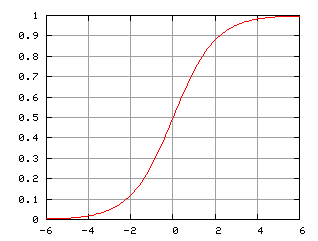
\includegraphics[width = 0.4\textwidth]{img/EcuacionLogistica.png}
\caption{Gráfica de $P(t) = \frac{1}{1+e^{-t}}$}
\label{fig:EcLogistica}
\end{figure}

\end{frame}

\subsection{Procesos de Verhulst.}

\begin{frame}
\framesubtitle{Modelo}
\begin{definition}[Proceso de Verhulst]
Modelo matemático que representa el desarrollo del número de individuos de una población a lo largo del tiempo.
\end{definition}

\textbf{Descripción del modelo}
\begin{itemize}
\item Ratio de crecimiento
\[R=\frac{x_{n+1}-x_n}{x_n}\]

\item Si $R=r$ constante
\[x_{n+1} = f(x_n) = (1+r)x_n\]
lo que os lleva a
\[x_n = (1+r)^nx_0\]

\item Verhulst mejora el modelo con
\[R=r(1-x_n)\]
obteniendo
\begin{equation}\label{eq:Verhulst}
x_{n+1} = f(x_n) = (1+r)x_n - rx_n^2
\end{equation}
\end{itemize}
\end{frame}

\begin{frame}
\framesubtitle{Puntos fijos}

\begin{block}{Punto fijo}
Un punto fijo de una función $f$ es aquel tal que
\[x=f(x)\]
\end{block}

\begin{itemize}
\item El punto fijo $x_0=0$ es estable.
\item El punto fijo $x_0=1$ requiere estudio
\begin{itemize}
\item Definimos el error
\[δ_n = x_n-1\]
\item Linealizando \eqref{eq:Verhulst} tenemos
\[δ_{n+1} = (1-r)δ_n\]
\item Vemos que la estabilidad depende de $r$.
\end{itemize}
\end{itemize}
\end{frame}

\begin{frame}
\framesubtitle{Estabilidad según $r$}

\begin{minipage}{0.32\textwidth}
\begin{figure}[hbtp]
\centering
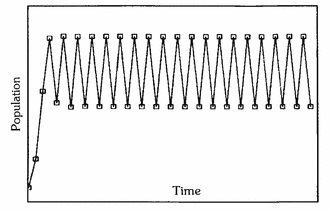
\includegraphics[width = \textwidth]{img/r2_3.png}
\caption{Evolución de la población con $r=2.3$}
\label{fig:r2_3}
\end{figure}
\end{minipage}
\begin{minipage}{0.32\textwidth}
\begin{figure}[hbtp]
\centering
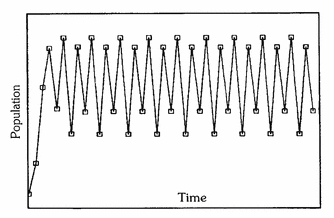
\includegraphics[width = \textwidth]{img/r2_5.png}
\caption{Evolución de la población con $r=2.5$}
\label{fig:r2_5}
\end{figure}
\end{minipage}
\begin{minipage}{0.32\textwidth}
\begin{figure}[hbtp]
\centering
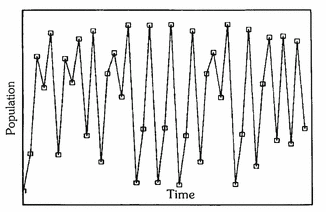
\includegraphics[width = \textwidth]{img/r3.png}
\caption{Evolución de la población con $r=3$}
\label{fig:r3}
\end{figure}
\end{minipage}
\end{frame}

\begin{frame}
\framesubtitle{Estabilidad}
\begin{figure}[hbtp]
\centering
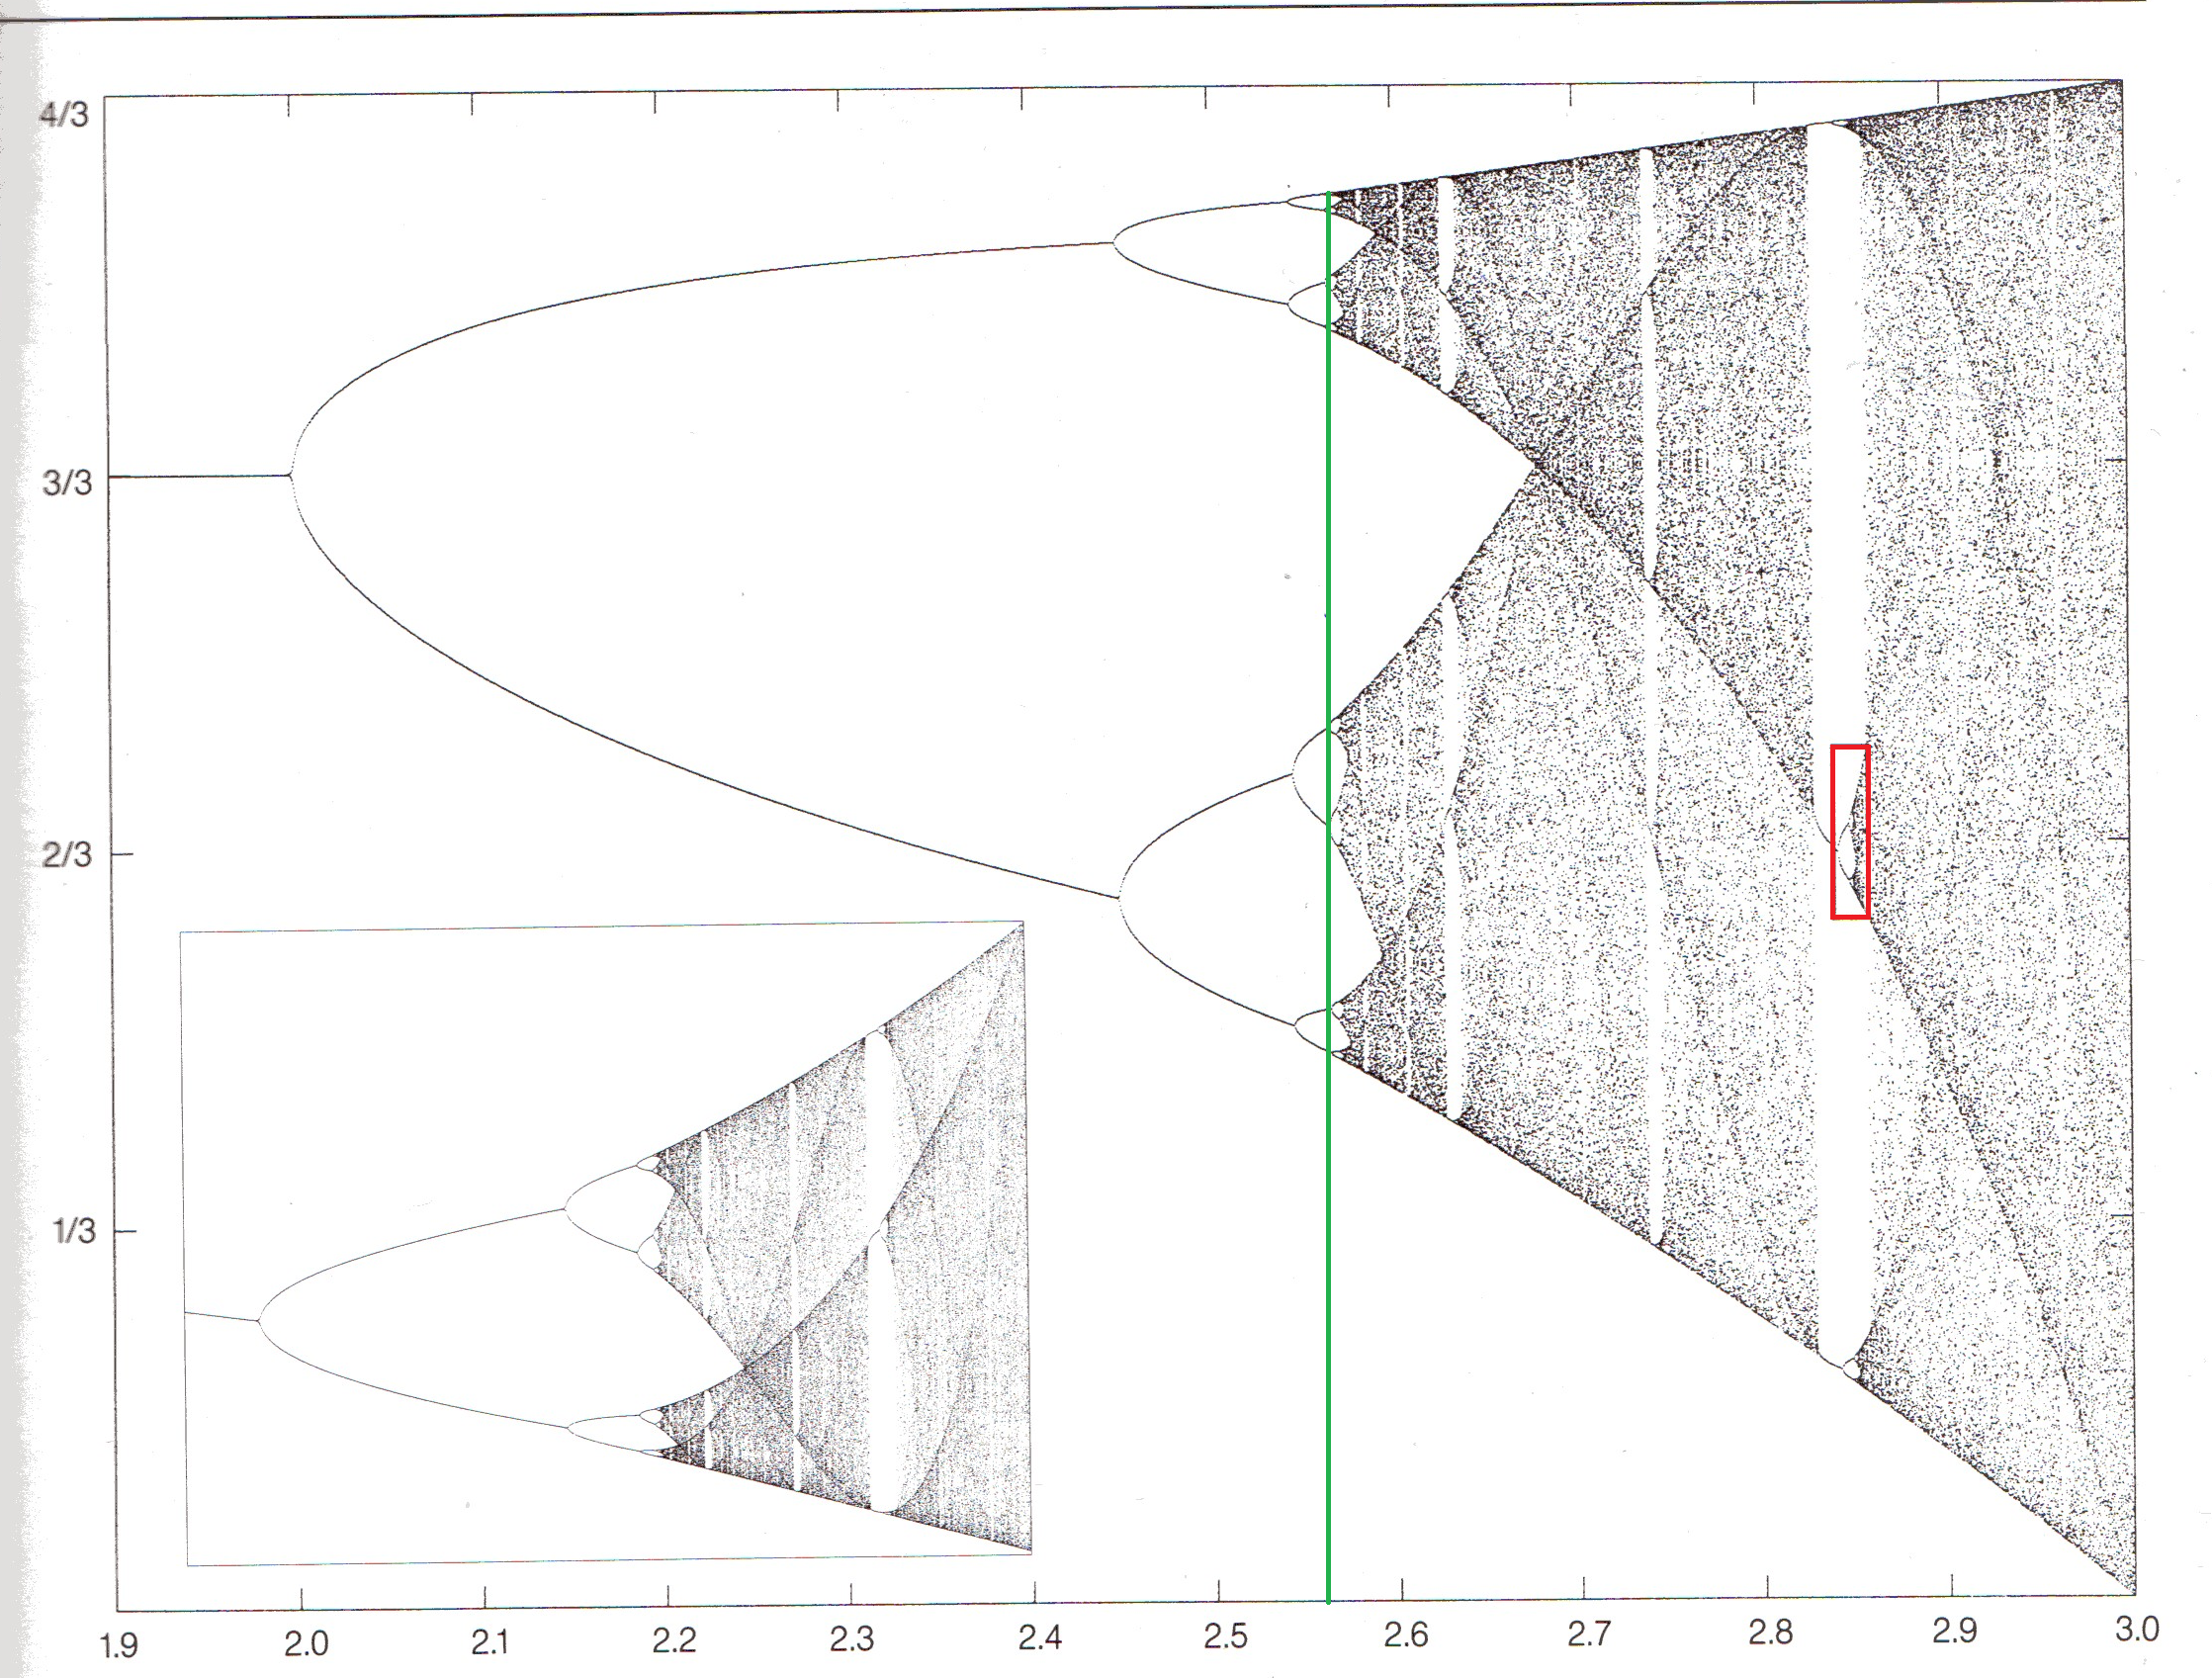
\includegraphics[width = 0.7 \textwidth]{img/verhulst6.png}
\caption{Visión global}
\label{fig:global}
\end{figure}
\end{frame}

\subsection{Conjuntos de Julia y Mandelbrot}

\begin{frame}
\framesubtitle{Repaso de números complejos}

Es necesario tener claras las ideas básicas de los números complejos para hablar de los conjuntos de Julia y Mandelbrot.

\begin{itemize}
\item Son números de la forma
\[z=a +bi\]
donde $a$ y $b$ son números reales e $i=\sqrt{-1}$
\item Se representan como puntos de un plano: \textbf{el plano complejo}

Cada número complejo tiene asociado un punto del plano y viceversa

\item Á menudo nos interesará considerar su módulo:
\[|z| = \sqrt{a^2+b^2}\]
\end{itemize}

\end{frame}

\subsubsection{Conjunto de Julia}

\begin{frame}
\begin{block}{Conjunto de Julia}
Familia de conjuntos fractales que se obtienen al estudiar el comportamiento de los números complejos al ser iterados por una función.

Iterando en la siguiente \ref{eq:Julia} con $c$ constante obtenemos un ejemplo de conjunto de Julia

\begin{equation}
z_{n+1} = z_n^2+c \text{ siendo } c \text{ un número complejo}
\end{equation}\label{eq:Julia}
\end{block}

Para generarlo consideramos la iteración

\begin{minipage}{0.3\textwidth}
\[\begin{array}{l}
z_0=z_0\\
z_1=z_0^2+c \\
z_2 = z_1^2 + c \\
\vdots \\
z_{n+1} = z_n^2+c
\end{array}\]
\end{minipage}
\begin{minipage}{0.68\textwidth}
\begin{figure}[hbtp]
\centering
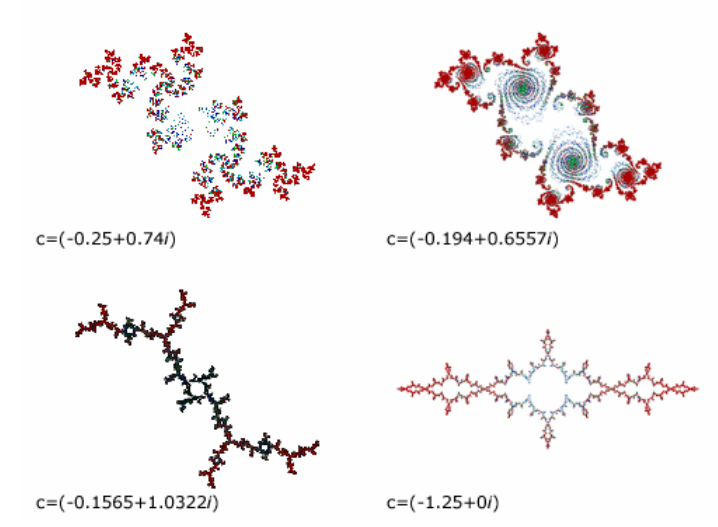
\includegraphics[width = 0.6\textwidth]{img/Julia_sets.png}
\caption{Ejemplos de conjuntos de Julia}
\label{fig:Julia}
\end{figure}
\end{minipage}
\end{frame}

\subsubsection{Conjunto de Mandelbrot}

\begin{frame}
\begin{block}{Conjunto de Mandelbrot}
Mandelbrot modifica el proceso iterativo de Julia haciendo variable el punto $c$ y fijando el punto $z_0=0$.
\end{block}

El conjunto de Mandelbrot es el conjunto de números complejos $c$ para los cuales la sucesión de puntos obtenida por el método iterativo:

\begin{minipage}{0.3\textwidth}
\[\begin{array}{l}
z_0=z_0\\
z_1=z_0^2+c \\
z_2 = z_1^2 + c \\
\vdots \\
z_{n+1} = z_n^2+c
\end{array}\]
no tiende a infinito, es decir, está acotada.
\end{minipage}
\begin{minipage}{0.68\textwidth}
\begin{figure}[hbtp]
\centering

\includegraphics[width = 0.6\textwidth]{img/Mandelbrot_set.png}
\caption{Conjunto de Mandelbrot}
\label{fig:Mandelbrot}
\end{figure}
\end{minipage}
\end{frame}

\subsection{Fractales, dimensión de Hausdorlf y dimensión fractal}

\begin{frame}
\begin{itemize}
\item El término fractal fue propuesto por el matemático \textbf{Benoit Mandelbrot} en 1975, procedente del latin ``Fractus'' que significa ``fracturado''.
\item Recordemos que en la figura \ref{fig:Mandelbrot} la diferencia entre los distintos colores mostrados se debía a la convergencia o no de los diferentes puntos del plano al aplicarles la ecuación de Mandelbrot.
\item La relación entre el caos y los fractales se da en la frontera del dibujo.
\end{itemize}

\begin{minipage}{0.48\textwidth}
\begin{figure}[hbtp]
\centering
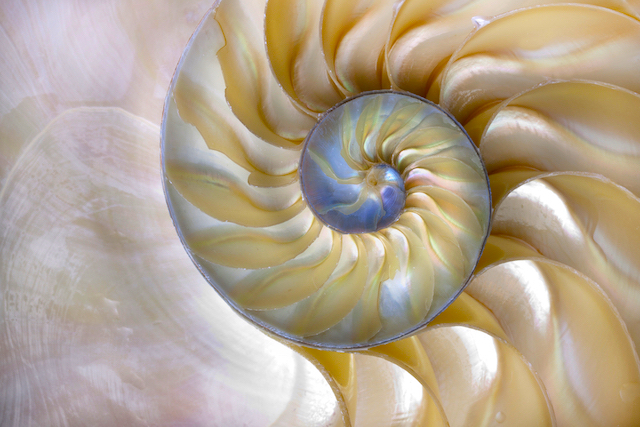
\includegraphics[width = 0.6\textwidth]{img/concha.jpg}
\caption{Concha de un molusco}
\label{fig:concha}
\end{figure}
\end{minipage}
\begin{minipage}{0.48\textwidth}
\begin{figure}[hbtp]
\centering
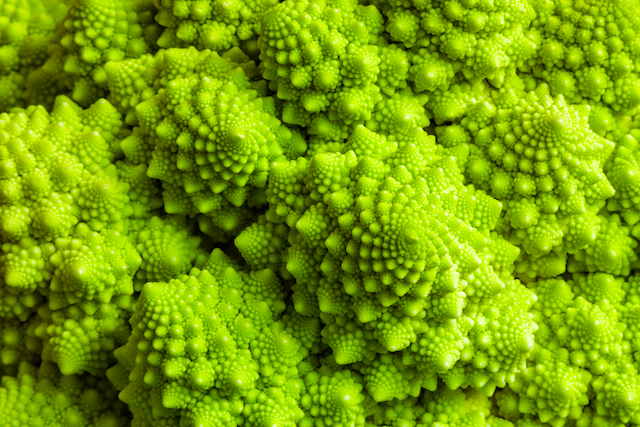
\includegraphics[width = 0.6\textwidth]{img/brocoli.jpg}
\caption{Trozo de brocoli al que se ha aplicado zoom}
\label{fig:brocoli}
\end{figure}
\end{minipage}

\begin{itemize}
\item La existencia de los fractales en la vida cotidiana se debe a la gran capacidad de comprimir información que tienen asociada.
\item Definición recursiva de árbol.
\end{itemize}

\end{frame}

\subsection{Polvo de Cantor}

\begin{frame}
\begin{block}{Polvo de Cantor}
Se denomina Polvo de Cantor al fractal resultante de iterar sobre el conjunto de cantor en dos dimensiones.
\end{block}

\begin{block}{Conjunto de Cantor}
Conjunto construido mediante el siguiente proceso:

\begin{enumerate}
\item Tomamos el intervalo [0,1], lo dividimos en 3 intervalos iguales y eliminamos el intervalo central

\item Volvemos al paso 1 sobre cada uno de los dos conjuntos restantes.
\end{enumerate}

La imagen \ref{fig:conjuntoCantor} ilustra la construcción de este conjunto.
\end{block}

\begin{figure}[hbtp]
\centering
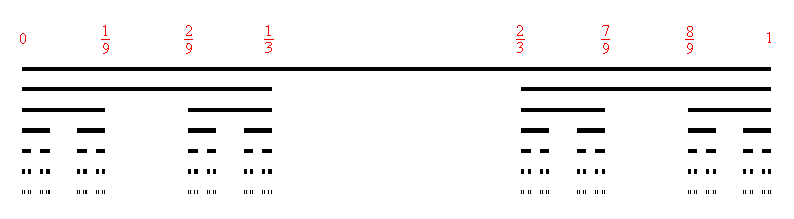
\includegraphics[width = 0.7\textwidth]{img/conjuntoCantor.png}
\caption{Primeras etapas del proceso de construcción del conjunto de Cantor}
\label{fig:conjuntoCantor}
\end{figure}

\end{frame}

\section{Sistemas continuos}
\subsection{Sistemas dinámicos deterministas, ecuaciones diferenciales}
\begin{frame}
\framesubtitle{Introducción}

\textbf{Comparación con ecuacines en diferencias:}
\begin{itemize}
\item La diferencia con los sistemas dinámicos en diferencias se debe a la continuidad de las variables
\item Expresamos los incrementos como derivadas
\item Obtenemos \textbf{ecuaciones diferenciales}
\end{itemize}

\begin{block}{Ecuación diferencial}
Una ecuación diferencial es una fórmula matemática que relaciona una función con sus derivadas.

Por ejemplo
\[y'(x) = y(x) \implies y(x) = e^{x+c}\]
\end{block}
\end{frame}

\begin{frame}
\framesubtitle{Ecuación del calor}

\begin{block}{Ecuación del calor}
La ecuación del calor es una importante ecuación diferencial en derivadas parciales del tipo parabólica que describe la distribución del calor (o variaciones de la temperatura) en una región a lo largo del transcurso del tiempo.
\end{block}

\textbf{Modelización del problema}
\begin{itemize}
\item La variable $t$ es el tiempo
\item Definimos $x(t)$ como la diferencia de temperatura en todo instante $t$
\item $x'(t)$ nos da la variación de temperatura en todo instante $t$
\item \textbf{Teoría:} La tasa de cambio de temperatura es inversamente proporcional a la diferencia de temperatura
\end{itemize}

La ecuación que modeliza este fenómeno es:
\begin{equation}
x'(t) = ax(t)~~~con~~ a<0
\end{equation}

Cuya solución viene dada por:
\begin{equation}
x(t) = c\cdot e^{at}
\end{equation}
\end{frame}

\begin{frame}
\framesubtitle{Péndulo}
\begin{block}{Movimiento del péndulo}
Queremos estudiar el movimiento de un péndulo que tiene en su extremo un peso y que cuelga de un soporte que limita su movimiento a lo largo de un círculo.
\end{block}

\textbf{Modelización del sistema}
\begin{itemize}
\item La variable $t$ es el tiempo.
\item Definimos $x(t)$ como la posición angular del péndulo en todo instante $t$.
\item La función $x'(t)$ mide la velocidad angular del péndulo.
\item La función $x''(t)$ mide la aceleración angular del péndulo en todo instante $t$
\end{itemize}

La ecuación que modeliza este fenómeno es:
\begin{equation}
x''(t) = -\sin x(t)
\end{equation}

Se trata de una ecuación de \emph{segundo orden} y es una de las más importantes en ciencia.
\end{frame}

\begin{frame}
\framesubtitle{Clasificación de Ecuaciones Diferenciales Ordinarias}
\begin{itemize}
\item Según el orden de las derivadas que aparezcan en la expresión:
  \begin{itemize}
  \item Primer orden
  \item Segundo orden
  \item ...
  \end{itemize}
\item Según la relación entre la función $x$ y sus derivadas
  \begin{itemize}
  \item Lineales
  \item No lineales
  \end{itemize}
\item Según si aparece explicítamente la variable $t$ en la ecuación
  \begin{itemize}
  \item Autónomas
  \item No autónomas
  \end{itemize}
\end{itemize}
\end{frame}

\begin{frame}
\framesubtitle{Dependencia del dato inicial: Caos}

\begin{block}{Dependencia del dato inicial}
Siempre es necesario conocer un dato inicial a fin de determinar con exactitud la solución de la ecuación. Sin embargo, en ocasiones, pequeños errores al medir este dato inicial pueden dar lugar a grandes cambios en el sistema.
\end{block}

\begin{minipage}{0.48\textwidth}
\begin{center}
\begin{tikzpicture}
\begin{axis}[xmin=-1, xmax=1, samples=50, width=6cm, height=6cm, cycle list name=color list]
  \addplot (x,-7*e^x);
  \addplot (x,-6*e^x);
  \addplot (x,-5*e^x);
  \addplot (x,-3*e^x);
  \addplot (x,4*e^x);
  \addplot (x,-3*e^x);
  \addplot (x,-2*e^x);
  \addplot (x,-1*e^x);
  \addplot (x,e^x);
  \addplot (x,2*e^x);
  \addplot (x,3*e^x);
  \addplot (x,4*e^x);
  \addplot (x,5*e^x);
  \addplot (x,6*e^x);
  \addplot (x,7*e^x);
\end{axis}
\end{tikzpicture}
\captionof{figure}{Familia de funciones de la forma $x(t)=x(0)e^t$}
\end{center}
\end{minipage}
\begin{minipage}{0.48\textwidth}
\begin{center}
\begin{tikzpicture}
\begin{axis}[xmin=-1, xmax=1, samples=50, width=6cm, height=6cm, cycle list name=color list]
  \addplot (x,-7*e^-x);
  \addplot (x,-6*e^-x);
  \addplot (x,-5*e^-x);
  \addplot (x,-3*e^-x);
  \addplot (x,4*e^-x);
  \addplot (x,-3*e^-x);
  \addplot (x,-2*e^-x);
  \addplot (x,-1*e^-x);
  \addplot (x,e^-x);
  \addplot (x,2*e^-x);
  \addplot (x,3*e^-x);
  \addplot (x,4*e^-x);
  \addplot (x,5*e^-x);
  \addplot (x,6*e^-x);
  \addplot (x,7*e^-x);
\end{axis}
\end{tikzpicture}
\captionof{figure}{Familia de funciones de la forma $x(t)=x(0)e^{-t}$}
\end{center}
\end{minipage}
\end{frame}

\subsection{Espacio de estados/fases}

\begin{frame}
\begin{itemize}
\item A menudo no es nada sencillo obtener la solución de una ecuación diferencial.
\item En matemáticas hay una asignatura completa dedicada a la comprensión de estas ecuaciones.
\item Sin embargo puede estudiarse la tendencia general de la solución.
\item Para ello empleamos los \textbf{diagrama de fases}
\end{itemize}

\textbf{Consideramos un problema general $x'(t)=f(x(t))$}
\begin{figure}[hbtp]
\centering
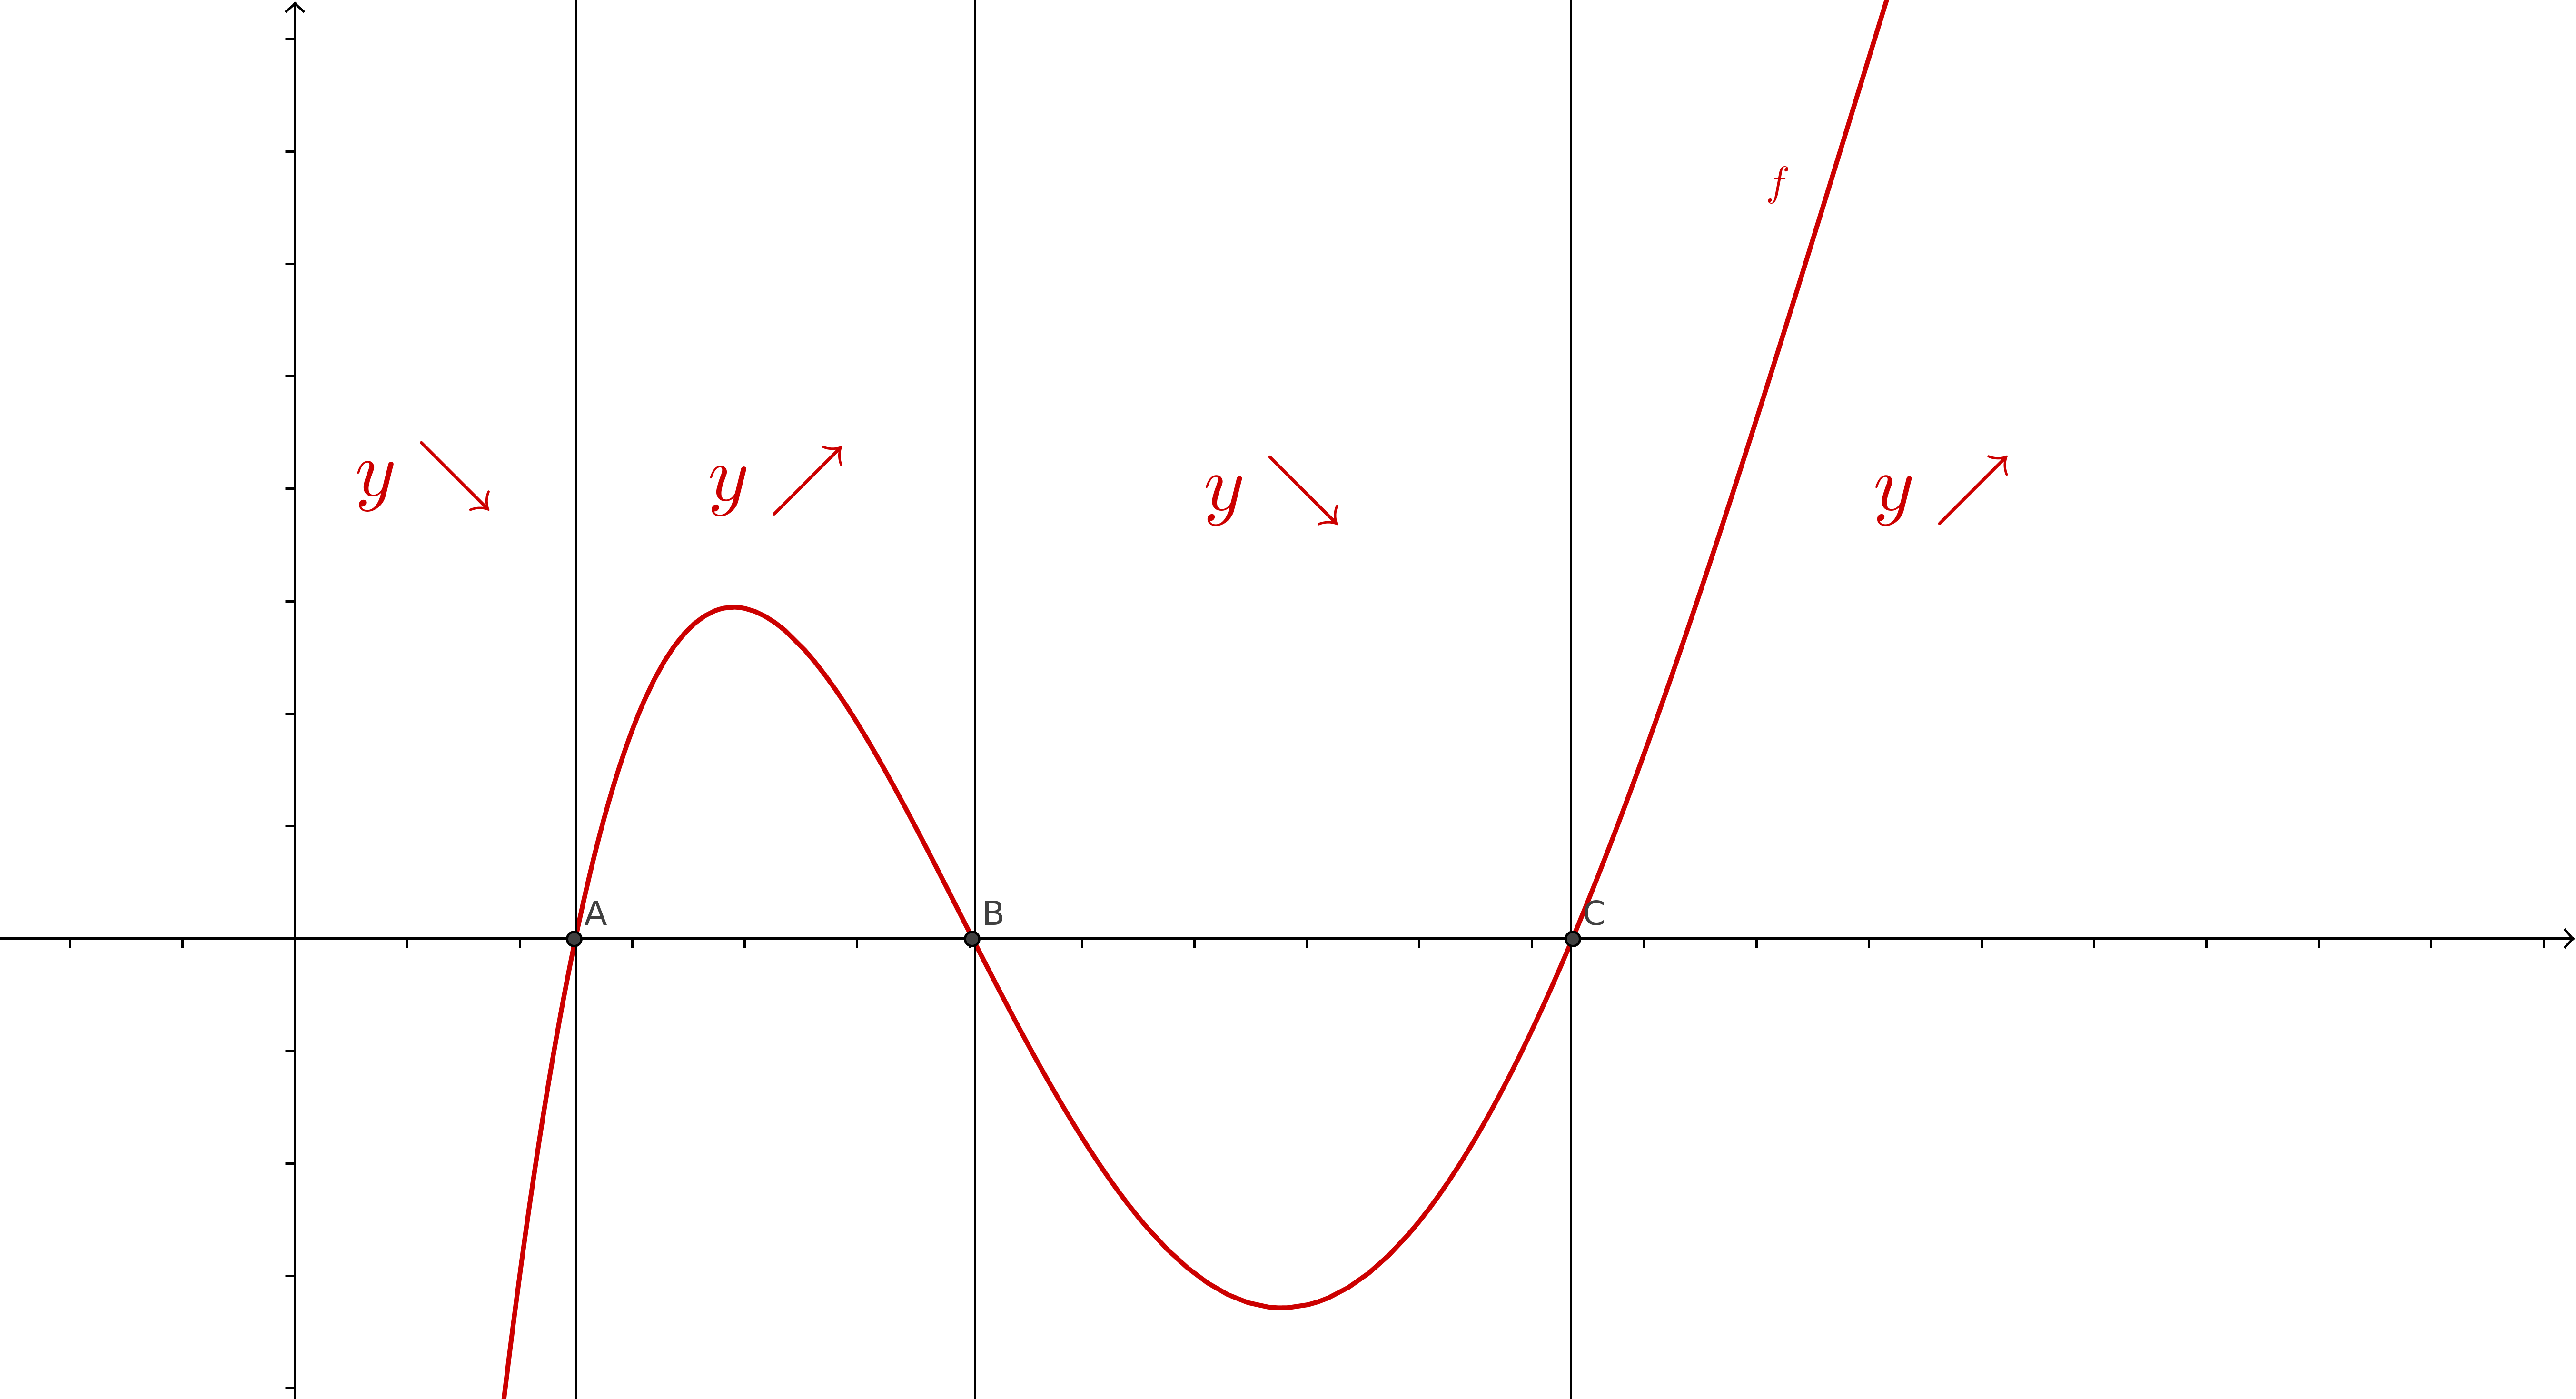
\includegraphics[width = 0.6\textwidth]{img/propiedades-autonomas.png}
\end{figure}

\begin{figure}[hbtp]
\centering
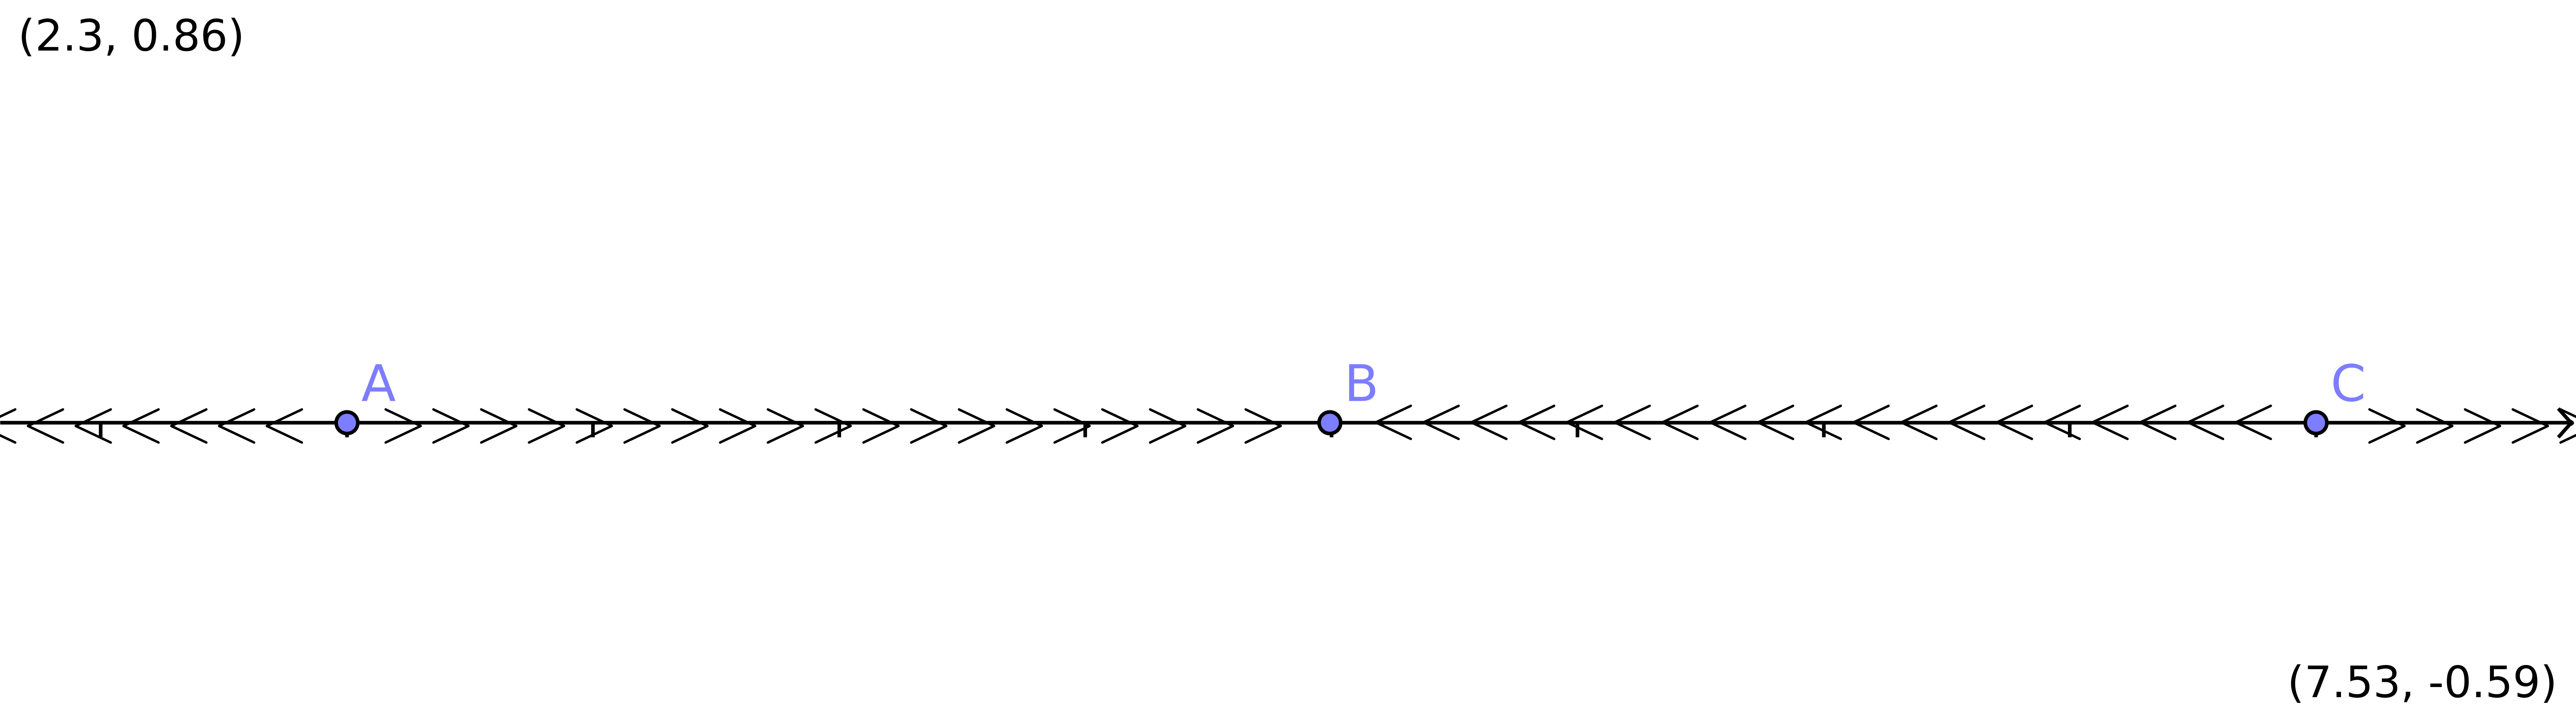
\includegraphics[width = 0.6\textwidth]{img/diagrama-fases.png}
\end{figure}

\end{frame}

\subsection{Oscilaciones}
\subsection{Sistemas disipativos: atractores}
\subsection{Flujos, compresibles o no}
\subsection{Atractores extraños: caos}
\subsection{Ejemplos de sistemas}
\subsection{Lorenz Volterra}

\subsection{Órbitas caóticas y exponentes de Lyapunov}

\begin{frame}
\framesubtitle{Definición}
\textbf{El concepto de equilibrio inestable es muy común en física}

\begin{example}
Aunque en teoría podemos colocar una pelota en el pico de una montaña sin que se mueva, en la práctica esto es imposible.

El estado de equilibrio estático es \textbf{inestable}
\end{example}

Un comportamiento muy común en algunos sistemas dinámicos es pasar de un estado de equilibrio inestable a otro estable.

\begin{block}{Órbitas caóticas}
Las órbitas caóticas son aquellas que permanecen siempre en un estado inestable, sin llegar a ser converger o ser atraídas hacia níngun estado estático o periódico estable.

Esta irregularidad es cuantificada mediante los \textbf{números de Lyapunov} y los \textbf{exponentes de Lyapunov}.
\end{block}

\begin{block}{Número de Lyapunov}
Informalmente, diremos que el \textbf{número de Lyapunov} es la tasa o razón media a la que los puntos divergen a lo largo de la órbita. Diremos que el \textbf{exponente de Lyapunov} es el logaritmo natural del número de Lyapunov.
\end{block}

\end{frame}

\begin{frame}
\framesubtitle{Ejemplo numérico}

\begin{itemize}
\item Encontramos \emph{caos} cuando los coeficientes de Lyapunov de nuestro sistema dinámico son mayores que 1.
\end{itemize}

\begin{block}{Exponente de Lyapunov (definición formal)}
Dado un dato inicial $x_0$ consideramos un dato cercano $x_0+ε_0$, como ya hicimos en el ejemplo \ref{example:Julia} siendo la separación $ε_0$ extremadamente pequeña.

Sea $ε_n$ la separación tras $n$ iteraciones, si se da la relación $|ε_n|\approx e^{n\cdot λ}|ε_0|$, decimos que λ es el \textbf{exponente de Lyapunov}.
\end{block}

\begin{example}
Vamos a calcular el exponente de Lyapunov para el caso concreto
\[f(x) = \left\{ \begin{array}{ll}
rx, & 0 \leq x \leq \frac{1}{2}\\
r-rx, & \frac{1}{2} < x \leq 1
\end{array}\right.\]

De forma genérica tendremos:
\[ε_n = f^n(x_0+ε_0)-f^n(x_0) \]
y queremos escribir
\[|ε_n| = |ε_0| e^{nλ} \implies λ = \frac{1}{n} \ln\left| \frac{ε_n}{ε_0}\right| = \frac{1}{n}\ln \left|\frac{f^n(x_0+ε_0)-f^n(x_0)}{ε_0} \right| = \frac{1}{n}\ln \left|(f^n)'(x_0) \right|\]
\end{example}
\end{frame}

\begin{frame}
\framesubtitle{Ejemplo numérico}
\begin{example}[Continuación]
donde en el último paso hemos considerado $ε_0 \to 0$.

Aplicando la regla de la cadena podemos escribir
\[(f^n)'(x_0) = \prod_{i=0}^{n-1}f'(x_i) \]

Razonando sobre los multiplicadores podemos escribir
\[\ln \left|\prod_{i=0}^{n-1}f'(x_i)\right| = \sum{i=0}^{n-1}\ln |f'(x_i)| \]

En esta ocasión tenemos $f'(x)=\pm r$ para todo $x$ lo que nos lleva a
\[λ= \frac{1}{n}\sum_{i=0}^{n-1}\ln |f'(x_i)| = \ln r\]
\end{example}
\end{frame}

\section{Aplicaciones}
\subsection{Generación gráfica de conjuntos de Julia}
\subsection{Ejemplos gráficos de explorar el conjunto de Mandelbrot}
\subsection{Caos y criptografía}
\subsection{Compresión fractal}
\subsection{Antenas fractales}

\begin{frame}
Las transparencias que vienen a continuación son las que aparecen por defecto con el paquete que estamos usando. Las dejamos hasta el último momento ya que ahí se pueden ver muchos ejemplos de cómo hacer diferentes cosas.

El índice no se ve bien ahora mismo. Pasemos de eso, cuando tengamos esto terminado y veamos cuántas secciones y subsecciones hemos utilizado nos peleamos con cómo mostrar el índice.
\end{frame}



\begin{frame}
\frametitle{Overview} % Table of contents slide, comment this block out to remove it
\tableofcontents % Throughout your presentation, if you choose to use \section{} and \subsection{} commands, these will automatically be printed on this slide as an overview of your presentation
\end{frame}


%----------------------------------------------------------------------------------------
%	PRESENTATION SLIDES
%----------------------------------------------------------------------------------------

%------------------------------------------------
\section{First Section} % Sections can be created in order to organize your presentation into discrete blocks, all sections and subsections are automatically printed in the table of contents as an overview of the talk
%------------------------------------------------

\subsection{Subsection Example} % A subsection can be created just before a set of slides with a common theme to further break down your presentation into chunks

\begin{frame}
\frametitle{Paragraphs of Text}
Sed iaculis dapibus gravida. Morbi sed tortor erat, nec interdum arcu. Sed id lorem lectus. Quisque viverra augue id sem ornare non aliquam nibh tristique. Aenean in ligula nisl. Nulla sed tellus ipsum. Donec vestibulum ligula non lorem vulputate fermentum accumsan neque mollis.\\~\\

Sed diam enim, sagittis nec condimentum sit amet, ullamcorper sit amet libero. Aliquam vel dui orci, a porta odio. Nullam id suscipit ipsum. Aenean lobortis commodo sem, ut commodo leo gravida vitae. Pellentesque vehicula ante iaculis arcu pretium rutrum eget sit amet purus. Integer ornare nulla quis neque ultrices lobortis. Vestibulum ultrices tincidunt libero, quis commodo erat ullamcorper id.
\end{frame}

%------------------------------------------------

\begin{frame}
\frametitle{Bullet Points}
\begin{itemize}
\item Lorem ipsum dolor sit amet, consectetur adipiscing elit
\item Aliquam blandit faucibus nisi, sit amet dapibus enim tempus eu
\item Nulla commodo, erat quis gravida posuere, elit lacus lobortis est, quis porttitor odio mauris at libero
\item Nam cursus est eget velit posuere pellentesque
\item Vestibulum faucibus velit a augue condimentum quis convallis nulla gravida
\end{itemize}
\end{frame}

%------------------------------------------------

\begin{frame}
\frametitle{Blocks of Highlighted Text}
\begin{block}{Block 1}
Lorem ipsum dolor sit amet, consectetur adipiscing elit. Integer lectus nisl, ultricies in feugiat rutrum, porttitor sit amet augue. Aliquam ut tortor mauris. Sed volutpat ante purus, quis accumsan dolor.
\end{block}

\begin{block}{Block 2}
Pellentesque sed tellus purus. Class aptent taciti sociosqu ad litora torquent per conubia nostra, per inceptos himenaeos. Vestibulum quis magna at risus dictum tempor eu vitae velit.
\end{block}

\begin{block}{Block 3}
Suspendisse tincidunt sagittis gravida. Curabitur condimentum, enim sed venenatis rutrum, ipsum neque consectetur orci, sed blandit justo nisi ac lacus.
\end{block}
\end{frame}

%------------------------------------------------

\begin{frame}
\frametitle{Multiple Columns}
\begin{columns}[c] % The "c" option specifies centered vertical alignment while the "t" option is used for top vertical alignment

\column{.45\textwidth} % Left column and width
\textbf{Heading}
\begin{enumerate}
\item Statement
\item Explanation
\item Example
\end{enumerate}

\column{.5\textwidth} % Right column and width
Lorem ipsum dolor sit amet, consectetur adipiscing elit. Integer lectus nisl, ultricies in feugiat rutrum, porttitor sit amet augue. Aliquam ut tortor mauris. Sed volutpat ante purus, quis accumsan dolor.

\end{columns}
\end{frame}

%------------------------------------------------
\section{Second Section}
%------------------------------------------------

\begin{frame}
\frametitle{Table}
\begin{table}
\begin{tabular}{l l l}
\toprule
\textbf{Treatments} & \textbf{Response 1} & \textbf{Response 2}\\
\midrule
Treatment 1 & 0.0003262 & 0.562 \\
Treatment 2 & 0.0015681 & 0.910 \\
Treatment 3 & 0.0009271 & 0.296 \\
\bottomrule
\end{tabular}
\caption{Table caption}
\end{table}
\end{frame}

%------------------------------------------------

\begin{frame}
\frametitle{Theorem}
\begin{theorem}[Mass--energy equivalence]
$E = mc^2$
\end{theorem}
\end{frame}

%------------------------------------------------

\begin{frame}[fragile] % Need to use the fragile option when verbatim is used in the slide
\frametitle{Verbatim}
\begin{example}[Theorem Slide Code]
\begin{verbatim}
\begin{frame}
\frametitle{Theorem}
\begin{theorem}[Mass--energy equivalence]
$E = mc^2$
\end{theorem}
\end{frame}\end{verbatim}
\end{example}
\end{frame}

%------------------------------------------------

\begin{frame}
\frametitle{Figure}
Uncomment the code on this slide to include your own image from the same directory as the template .TeX file.
%\begin{figure}
%\includegraphics[width=0.8\linewidth]{test}
%\end{figure}
\end{frame}

%------------------------------------------------

\begin{frame}[fragile] % Need to use the fragile option when verbatim is used in the slide
\frametitle{Citation}
An example of the \verb|\cite| command to cite within the presentation:\\~

This statement requires citation \cite{p1}.
\end{frame}

%------------------------------------------------

\begin{frame}
\frametitle{References}
\footnotesize{
\begin{thebibliography}{99} % Beamer does not support BibTeX so references must be inserted manually as below
\bibitem[Smith, 2012]{p1} John Smith (2012)
\newblock Title of the publication
\newblock \emph{Journal Name} 12(3), 45 -- 678.
\end{thebibliography}
}
\end{frame}

%------------------------------------------------

\begin{frame}
\Huge{\centerline{The End}}
\end{frame}

%----------------------------------------------------------------------------------------

\end{document}